\subsubsection{bringit::client::event::CompleteListEventEmitter}

\label{bringit::client::event::CompleteListEventEmitter}
\begin{figure}[H]
	\centering
	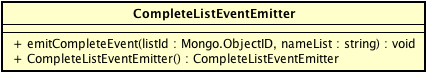
\includegraphics[scale=0.5]{Sezioni/SottosezioniST/img/app/CompleteListEventEmitter.png}
	\caption{bringit::client::event::CompleteListEventEmitter}
\end{figure}

\begin{itemize}
\item \textbf{Descrizione}: Classe per l'emissione dell'evento relativo al completamento della lista bringit.
\item \textbf{Utilizzo}: La classe viene usata quando la lista viene completata, emettendo l'evento completeEvent.
\item \textbf{Attributi}: 
\item \textbf{Metodi}:
	\begin{itemize}
	\item \textit{public CompleteListEventEmitter():CompleteListEventEmitter}\\
	Il costruttore della classe CompleteListEventEmitter.
	\item \textit{public emitCompleteEvent(listId:string,nameList:string):void}\\
	Questo metodo emette l'evento del completamento della lista.
					\\ \textbf{Parametri}: \begin{itemize}
			\item \textit{listId:string}\\
			L'identificativo della lista che è stata completata.
			\item \textit{nameList:string}\\
			Il nome della lista che è stata completata.
					\end{itemize}
	\end{itemize}
\end{itemize}


\subsubsection{bringit::client::event::DeleteItemEventEmitter}

\label{bringit::client::event::DeleteItemEventEmitter}
\begin{figure}[H]
	\centering
	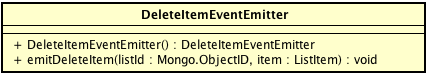
\includegraphics[scale=0.5]{Sezioni/SottosezioniST/img/app/DeleteItemEventEmitter.png}
	\caption{bringit::client::event::DeleteItemEventEmitter}
\end{figure}

\begin{itemize}
\item \textbf{Descrizione}: Classe per l'emissione dell'evento relativo all'eliminazione di un item della lista bringit.
\item \textbf{Utilizzo}: La classe viene usata quando un elemento della lista viene eliminato, emettendo un evento deleteEvent.
\item \textbf{Attributi}: 
\item \textbf{Metodi}:
	\begin{itemize}
	\item \textit{public DeleteItemEventEmitter():DeleteItemEventEmitter}\\
	Il costruttore della classe DeleteItemEventEmitter. 
	\item \textit{public emitDeleteItem(listId:string,item:ListItem):void}\\
	Questo metodo emette l'evento relativo all'eliminazione di un elemento della lista.
					\\ \textbf{Parametri}: \begin{itemize}
			\item \textit{listId:string}\\
			L'identificativo della lista dalla quale viene eliminato un item.
			\item \textit{item:ListItem}\\
			L'item che viene eliminato.
					\end{itemize}
	\end{itemize}
\end{itemize}


\subsubsection{bringit::client::event::DeleteListEmitter}

\label{bringit::client::event::DeleteListEmitter}
\begin{figure}[H]
	\centering
	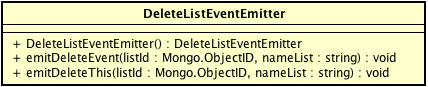
\includegraphics[scale=0.5]{Sezioni/SottosezioniST/img/app/DeleteListEmitter.png}
	\caption{bringit::client::event::DeleteListEmitter}
\end{figure}

\begin{itemize}
\item \textbf{Descrizione}: Classe per l'emissione dell'evento relativo all'eliminazione di una lista bringit.
\item \textbf{Utilizzo}: La classe viene usata quando una lista viene eliminata, emettendo un evento deleteEvent.
\item \textbf{Attributi}: 
\item \textbf{Metodi}:
	\begin{itemize}
	\item \textit{public DeleteListEmitter():DeleteListEmitter}\\
	Il costruttore della classe DeleteListEmitter.
	\item \textit{public emitDeleteEvent(listId:string,nameList:string):void}\\
	Questo metodo emette l'evento relativo all'eliminazione di una lista quando viene eliminata utilizzando l'apposito modale di conferma eliminazione.
					\\ \textbf{Parametri}: \begin{itemize}
			\item \textit{listId:string}\\
			L'identificativo della lista che viene eliminata.
			\item \textit{nameList:string}\\
			Il nome della lista che viene eliminata.
					\end{itemize}
					
	\item \textit{public emitDeleteThis(listId:string,item:ListItem):void}\\
	Questo metodo emette l'evento relativo all'eliminazione di una lista quando viene cliccato il messageActionButton.
					\\ \textbf{Parametri}: \begin{itemize}
			\item \textit{listId:string}\\
			L'identificativo della lista dalla quale viene eliminato un item.
			\item \textit{nameList:string}\\
			L'item che viene eliminato.
					\end{itemize}
	\end{itemize}
\item \textbf{Eventi}:
\end{itemize}

\subsubsection{bringit::client::event::ModifyListEventEmitter}

\label{bringit::client::event::ModifyListEventEmitter}
\begin{figure}[H]
	\centering
	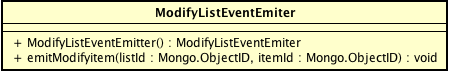
\includegraphics[scale=0.5]{Sezioni/SottosezioniST/img/app/ModifyListEventEmitter.png}
	\caption{bringit::client::event::ModifyListEventEmitter}
\end{figure}

\begin{itemize}
\item \textbf{Descrizione}: Classe per l'emissione dell'evento relativo alla modifica di un item di una lista bringit.
\item \textbf{Utilizzo}: La classe viene usata quando un item di una lista viene modificato, emettendo un evento modifyItem.
\item \textbf{Attributi}: 
\item \textbf{Metodi}:
	\begin{itemize}
	\item \textit{public ModifyListEventEmitter():ModifyListEventEmitter}\\
	Il costruttore della classe ModifyListEventEmitter.
	\item \textit{public emitModifyItem(listId:string,itemId:string):void}\\
	Questo metodo emette l'evento relativo alla modifica di un elemento della lista.
					\\ \textbf{Parametri}: \begin{itemize}
			\item \textit{listId:string}\\
			L'identificativo della lista della quale viene modificato un item.
			\item \textit{itemId:string}\\
			L'identificativo dell'item che viene modificato.
					\end{itemize}
	\end{itemize}
\end{itemize}

\subsubsection{bringit::client::event::SaveItemEventEmitter}

\label{bringit::client::event::SaveItemEventEmitter}
\begin{figure}[H]
	\centering
	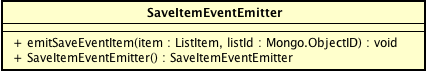
\includegraphics[scale=0.5]{Sezioni/SottosezioniST/img/app/SaveItemEventEmitter.png}
	\caption{bringit::client::event::SaveItemEventEmitter}
\end{figure}

\begin{itemize}
\item \textbf{Descrizione}: Classe per l'emissione dell'evento relativo al salvataggio di un item di una lista bringit nel database. 
\item \textbf{Utilizzo}: La classe viene usata quando un item di una lista viene salvato, emettendo un evento saveEventItem.
\item \textbf{Attributi}: 
\item \textbf{Metodi}:
	\begin{itemize}
	\item \textit{public SaveItemEventEmitter():SaveItemEventEmitter}\\
	Il costruttore della classe SaveItemEventEmitter.
	\item \textit{public emitSaveEventItem(listId:string,item:ListItem):void}\\
	Questo metodo emette l'evento relativo al salvataggio di un elemento della lista nel database.
					\\ \textbf{Parametri}: \begin{itemize}
			\item \textit{listId:string}\\
			L'identificativo della lista della quale viene modificato un item.
			\item \textit{item:ListItem}\\
			L'item che viene salvato.
					\end{itemize}
	\end{itemize}
\end{itemize}

\subsubsection{bringit::client::event::SaveListEventEmitter}

\label{bringit::client::event::SaveListEventEmitter}
\begin{figure}[H]
	\centering
	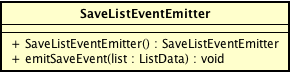
\includegraphics[scale=0.5]{Sezioni/SottosezioniST/img/app/SaveListEventEmitter.png}
	\caption{bringit::client::event::SaveListEventEmitter}
\end{figure}

\begin{itemize}
\item \textbf{Descrizione}: Classe per l'emissione dell'evento relativo al salvataggio di una lista bringit nel database. 
\item \textbf{Utilizzo}: La classe viene usata quando una lista viene salvata, emettendo un evento saveEvent.
\item \textbf{Attributi}: 
\item \textbf{Metodi}:
	\begin{itemize}
	\item \textit{public SaveListEventEmitter():SaveListEventEmitter}\\
	Il costruttore della classe SaveListEventEmitter.
	\item \textit{public emitSaveEvent(list:ListData):void}\\
	Questo metodo emette l'evento relativo al salvataggio di una lista nel database.
					\\ \textbf{Parametri}: \begin{itemize}
			\item \textit{list:ListData}\\
			La lista che viene salvata.
					\end{itemize}
	\end{itemize}
\end{itemize}

\subsubsection{bringit::client::event::ShareEventEmitter}

\label{bringit::client::event::ShareEventEmitter}
\begin{figure}[H]
	\centering
	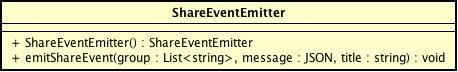
\includegraphics[scale=0.5]{Sezioni/SottosezioniST/img/app/ShareEventEmitter.png}
	\caption{bringit::client::event::ShareEventEmitter}
\end{figure}

\begin{itemize}
\item \textbf{Descrizione}: Classe per l'emissione dell'evento relativo alla condivisione di una lista bringit.
\item \textbf{Utilizzo}: La classe viene usata quando una lista viene condivisa, emettendo un evento shareEvent.
\item \textbf{Attributi}: 
\item \textbf{Metodi}:
	\begin{itemize}
	\item \textit{public ShareEventEmitter():ShareEventEmitter}\\
	Il costruttore della classe ShareEventEmitter.
	\item \textit{public emitShareEvent(group:,message:,title:string):void}\\
	Questo metodo emette l'evento relativo alla condivisione di una lista bringit.
					\\ \textbf{Parametri}: \begin{itemize}
			\item \textit{group:}\\
			
			\item \textit{message:}\\
			
			\item \textit{title:string}\\
			
					\end{itemize}
	\end{itemize}
\end{itemize}